\nonstopmode

\documentclass
[
    a4paper,
    twoside,
    12pt
]
{report}
\usepackage[utf8]{inputenc}
\renewcommand{\familydefault}{\rmdefault}
\usepackage[a4paper, left=3.19cm, right=3.19cm, top=2.54cm, bottom=2.54cm]{geometry}
\usepackage[american]{babel}
\usepackage{csquotes}
\usepackage{float}
\usepackage{enumerate}
\usepackage[bottom]{footmisc}
\usepackage{array}
\usepackage{ntheorem}
\usepackage{parskip}
\usepackage[right]{eurosym}
\usepackage{xcolor}
\usepackage[hyphens]{url}
\usepackage{makeidx}
\usepackage{multicol}
\usepackage{theorem}
\usepackage{listings}
\usepackage{graphicx}
\usepackage{pgfplots}
\pgfplotsset{compat=1.5}
\usepackage{csvsimple}
\usepackage{fancyhdr}
\usepackage{colortbl}
\usepackage{bchart}
\usepackage[hidelinks]{hyperref}
\usepackage{setspace}
\usepackage{mathptmx}
%\usepackage{showframe}
\pagestyle{plain}
\rhead{\thepage}
\sloppy

\usepackage[
backend=biber,
style=apa,
citestyle=authoryear
]{biblatex}

\addbibresource{references.bib}
\DeclareLanguageMapping{american}{american-apa}

%\setlength{\unitlength}{1cm}
%\setlength{\oddsidemargin}{0.3cm}
%\setlength{\evensidemargin}{0.3cm}
%\setlength{\textwidth}{15.5cm}
%\setlength{\topmargin}{-1.2cm}
%\setlength{\textheight}{24.7cm}
%\columnsep 0.5cm

%\title{Seminararbeit}
\selectcolormodel{gray}{

\newcommand{\Arbeitstitel}
	{
  	Success factors of video game consoles
	}
\newcommand{\Autor}
	{
		Dipl.-Ing. (FH) Lars Bartschat
	}

\newcommand{\MatrikelNr}
	{
		WBPA140000250
	}

\newcommand{\EmailAdresse}
	{
		bartschat@mailbox.org
	}
\newcommand{\Arbeitsart}
	{
		Seminar Paper
	}
\newcommand{\Studiengang}
	{
		Marketing Executive Program
	}
\newcommand{\Hochschule}
	{
		University of Münster
	}
\newcommand{\Lehrstuhl}
	{
		Department of Marketing and Media Research
	}
\newcommand{\Themensteller}
	{
		Prof. Dr. T. Hennig-Thurau
	}
\newcommand{\Betreuer}
	{
		M. Sc. R. Behrens
	}
\newcommand{\Ausgabedatum}
	{
		17.10.2016
	}
\newcommand{\Abgabedatum}
	{
		28.11.2016
	}
\newcommand{\Ort}
	{
		Münster}
			
		
\newcommand{\link}[1]{\ref{#1} (S. \pageref{#1})}
\begin{document}

\begin{titlepage}
    \vspace*{1.0cm}
    \begin{center}
        \begin{Large}
        \textbf{A neural network-based approach to accent conversion} \\
        \end{Large}
        \vspace*{1.0cm}
        \textit{Kenny W. Lino} \\
        \vspace*{1.5cm}
        Msc. Dissertation \\
        \vspace*{0.5cm}
        \begin{figure}[H]
        \centering
        
\includegraphics[scale=0.15]{img/UM-coat-of-arms.png}
    	\end{figure}
       \vspace*{1.0cm}
       Department of Intelligent Computer Systems \\
       Faculty of Information and Communication Technology \\
       University of Malta \\
       2018 \\
       
       \vspace*{2.0cm}
	   Supervisors: \\
       Claudia Borg, Department of Artificial Intelligence, University of Malta \\
       Andrea De Marco, Institute of Space Sciences and Astronomy, University of Malta \\
       Eva Navas, Department of Communications Engineering, University of the Basque Country \\
       
       \vspace*{4.5cm}
       Submitted in partial fulfilment of the requirements for the Degree of \\
       European Master of Science in Human Language Science and Technology
    \end{center}



\end{titlepage}

\onehalfspacing
\pagenumbering{Roman}

\cleardoublepage

\begin{center}
  M.Sc (HLST) \\
  \uppercase{\textbf{Faculty of Information and \\
  Communication Technology \\ University of Malta \\ }}
  \vspace*{0.5cm}
  Declaration \\
\end{center}
  \vspace*{1.5cm}
        Plagiarism is defined as "the unacknowledged use, as one's own work, of work of another person, whether or not such work has been published" (Regulations Governing Conduct at Examinations, 1997, Regulation 1 (viii), University of Malta). \\

I, the undersigned, declare that the Master's dissertation submitted is my own work, except where acknowledged and referenced. \\

I understand that the penalties for making a false declaration may include, but are not limited to, loss of marks; cancellation of examination results; enforced suspension of studies; or expulsion from the degree programme. \\
       
       \vspace*{1.5cm}
	     Student Name: Kenny W. Lino \\
       Course Code: CSA5310 HLST Dissertation \\
       Title of work: A neural network-based approach to accent conversion \\

       \vspace*{1.0cm}
       Signature of Student: \\

       \vspace*{1.0cm}
       Date:

\newpage
\section*{Abstract}\addcontentsline{toc}{section}{Abstract}

With the emergence of the use of technology in language learning through
tools like Rosetta Stone and Duolingo, learners have slowly been given
more autonomy of their language learning projection. Although these
tools have allowed learners to tailor their learning to their own
liking, there is a gap between the available resources to assist those
that would like to improve their pronunciation. Previous research in the
intersection of language learning and speech technology has made efforts
to develop pronunciation training systems to address this problem, but
the systems themselves tend to have gaps due to the lack of appropriate
support for the users, especially in appropriately identifying errors
and providing sufficient feedback to help them correct their errors.

Some researchers have purported that alongside other forms of feedback
such as a visual articulatory representation, a voice conversion system
could serve as a potential feedback mechanism by helping learners
understand what their voice could sound like given the appropriate
changes. However, like pronunciation training systems, voice conversion
systems also faced many limitations especially in terms of the quality
which made them unrenderable as useful tools. With that said, recent
advances in speech technology using deep neural networks have become
increasingly successful in achieving better accuracy and quality in a
variety of tasks, allowing for the potential to return and address these
said gaps in quality and performance for voice conversion.

In this thesis, I aim to investigate these advancements in applying deep
neural networks to develop a voice conversion system that could
potentially serve as a feedback mechanism as a part of a larger
computer-based pronunciation training system. Specifically, I intend to
adapt the methodologies of Aryal and Gutizerrez-Osuna (2014) to set
forth an accent conversion system that strives to convert a source voice
into a target accent, leveraging neural network architectures in place
of Gaussian Mixture Models for conversion.
\cleardoublepage
\tableofcontents
\addcontentsline{toc}{section}{Contents}
\clearpage
\listoffigures
\addcontentsline{toc}{section}{List of Figures}

\section*{List of Abbreviations}\addcontentsline{toc}{section}{List of Abbreviations}\begin{tabular}{ll}
    CAPT    & Computer Assisted Pronunciation Training \\
    CP      & Critical Period \\
    L1/L2    & First and second language \\
    LSTM & Long-short term memory \\
    TTS   & Text-to-speech \\
    
\end{tabular}

\clearpage
\cleardoublepage
\pagenumbering{arabic} \setcounter{page}{1}

\chapter{Introduction}

Technology has continuously evolved to no bounds as witnessed by the
current successes enjoyed by the use of neural networks and the power of
current hardware, something perhaps predicted by Moore's Law who
proclaimed that computing power would double once every 18 months (and
then changed to 24 months) {[}CITE HERE{]}. {[}Mention something about
AI here{]}

We see the effects of neural networks throughout many subareas in
computer science, including that of natural language processing. In
fact, if we take a look at the number of publications involving neural
networks, it has exponentially compounded annually {[}CITE IMAGE
HERE{]}.

While technology has flourished and led to a number of new
state-of-the-art systems such as improvements in commercial speech
recognition and machine translation, it can be argued that these
benefits have not reached and innovated other areas outside of research
to the same extent. One such example that could benefit from modern
innovations is education. Although there have been small trends here and
there to create applications for educational use such as Duolingo for
language learning{[}EXAMPLES?{]}, in general it seems that education has
not evolved at the same rate as tech. In particular, pronunciation has
been a large standing challenge in language learning due to its complex
nature. Unlike grammar and vocabulary pronunciation can be challenging
to both learn and teach due to the lack of clarity on how to teach it.

\section{Research Questions}\label{research-questions}

In this thesis, I focus on investigating the following questions:

\begin{itemize}
\item
  How can we leverage recent advances in recent technologies (namely
  deep neural networks) to convert a speaker's voice into sounding like
  it was said with another accent?
\item
  What specific methodologies achieve the best similarity to the target
  accent and produce the most natural sounding audio?
\end{itemize}

\section{Thesis Overview}\label{thesis-overview}

The overview of the thesis is as follows:

In Chapter 2, I present the motivation for creating an accent converison
system by discussing previous findings in second language acquisition
research especially in relation to speech.
\cleardoublepage

\chapter{Background}

Before delving into previous literature and their relevance to this work
and the field of NLP/language learning as a whole, I detail a few
important concepts often used in speech technology in order to make the
current work more accessible to those unfamiliar with the area.

Describe: * Voice conversion * MFCCs * GMMs * i-vectors
\chapter{Literature Review}

In this section, I begin by providing a brief overview of second
language acquisition and education in order to motivate the usage of
technology in language learning. I then examine some previous research
in computer assisted pronunciation (CAPT) systems in order to motivate
discussion about voice conversion and accent conversion, where I detail
important pivotal work done in the area.

\section{Theoretical and educational
motivations}\label{theoretical-and-educational-motivations}

\label{sec:theo-edu} Linguists have long debated over the possibility of
whether second language (L2) learners (e.g.~adult learners) could ever
acquire a language to the extent of a native speaker. Some still cite
ideas like the Critical Period (CP) Hypothesis and neuroplasticity which
claims that learners cannot acquire language (at least as well as a
native speaker) after a certain point in time due to the loss of
plasticity in the brain \parencite{lenneberg1967,scovel1988}. This
theory has been particularly cited in reference to pronunciation,
perhaps due to the obvious difficultly in overcoming the L1 negative
transfer that many, if not all, language learners experience in speaking
a new language.

Since the emergence of the CP hypothesis, many researchers have come to
find evidence that suggest the contrary. In \textcite{lengeris2012}, we
are presented an overview of the interactions between factors that
affect second language acquisition such as age, linguistic experience,
and learning setting. Here, we find evidence of studies such as
\textcite{bongaerts1995}, which present a counterargument against the CP
hypothesis. In this study, they discovered through a foreign accent
rating study with Dutch learners of English that learners could be
perceived as \textit{indistinguishable} from native speakers. Other
researchers such as Flege have also found that there is no distinct
`cut-off' point like the CP suggests. Thus, while age may have some
effect on a speaker's pronunciation, there is no conclusive evidence to
say that the loss of plasticity in the brain leads to an inability to
acquire language. As \textcite{lengeris2012} states, evidence for the CP
hypothesis would require `a sharp drop-off in a learner's abilities',
and `all early L2 learners should achieve native-like performance' (and
vice versa). This is not to say that learners are not still deterred by
other aspects like their own L1, but this does highlight the potential
that learners could be taught pronunciation, given the right settings.

Aside from the issue of whether or not language learners could ever
achieve native-like performance, another question that arises is whether
or not there is even a \textit{need} for learners to aim so high. In
\textcite{munro1999}, they discuss the interaction between foreign
accent, comprehensibility and intelligibility and point out that the
goal for many L2 learners is to communicate and not necessarily sound
like a native speaker. They also conduct a study to prove that despite
the fact that some speakers may have what some consider a `heavy
accent', that this does not automatically mean that they are
unintelligible. They found in their study that errors in prosody tended
to affect the speakers' intelligibility the most, which underscores the
role of prosody in organizing our utterances.

While linguists make these discoveries and observations of L2 learning,
it seems that it takes a lot of effort for them to trickle down to the
foreign language classroom. In \textcite{darcy2012}, they find through a
small survey of 14 teachers that although teachers tend to find
pronunciation to be `very important', the majority do not teach it at
all. When asked why they do not teach it, they cited reasons such as
`time, a lack of training and the need for more guidance and
institutional support'. Even though the number of teachers surveyed may
be significantly small, this gives us a glimpse through the lens of what
language teachers themselves experience in relation to pronunciation. We
see that even though teachers would like to address it, this would
require a restructuring in their curriculum and training-- something
that would undoubtedly take even more time before students get more
pronunciation attention. Compounded with the issue of time and the fact
that not all learners need or want equal amount of pronunciation
training, it may be unlikely to see such change in second language
curriculum so soon.

This points to the potential solution of employing a technology-based
system to improve pronunciation as learners could individually address
their needs \textit{outside} of the classroom.

\section{Computer-assisted pronunciation training
systems}\label{computer-assisted-pronunciation-training-systems}

\label{sec:capt} With the improvements of technology and speech
processing, researchers have attempted to make a number of
computer-assisted pronunciation training (CAPT) systems. In general,
CAPT systems utilize some form of automatic speech recognition (ASR) to
record a speaker and compares their recordings (usually) with a native
speaker gold standard. They also usually include a feedback mechanism
with a combination of pitch contours, spectrograms or audio recordings
to help the user adjust their pronunciation.

In \textcite{neri2002}, we are presented with an overview of the
interaction between language pedagogy and CAPT systems. Here, we see
that aside from the classroom, there seems to be an issue in relating
the findings of linguistics/language pedagogy with technology. Part of
the reason, they suggest, stems from the fact that there are not `clear
guidelines' on how to adapt second language acquisition research and
thus many CAPT systems `fail to meet sound pedagogical requirements'.
They emphasize the need for the learners to have appropriate input,
output, and feedback and exhibit how the systems available at the time
were lacking. For example, they criticize some CAPT systems that were
prevalent at the time including systems like \textit{Pro-nunciation} and
the \textit{Tell Me More} series for utilizing feedback systems that
give the users feedback in waveforms and spectrograms, which cannot be
easily interpreted without training. Further, they argue that although
visual feedback has its merits, this kind of feedback suggests to the
user that their utterance must look close to what is shown on the
screen, which is not the case. An utterance can be pronounced perfectly
fine, but look completely different from a spectrogram, and
\textit{especially} a waveform due to the number of features represented
in each visualization, such as the intensity, which will indefinitely
vary from user to user and the given examplar. They conclude their
article by making it a point to discuss recommendations for CAPT
systems, by stating that they should integrate what has been found in
research from second language acquisition, and to train pronunciation in
a communicative manner to give context to the learners. They also point
to the problematic area of feedback and advise that systems provide more
easily interpretable feedback with both audio and visual information,
and propose that systems give exercises that are `realistic, varied, and
engaging'. Despite the fact that this article was published in 2002,
this article provides a sound basis in addressing the proper makings of
a successful CAPT system.

In another article by \textcite{eskenazi2009}, we are given a brief
review of technologies in CAPT systems, this time more focused from a
technical perspective. In particular, she gives attention to the
different CAPT system types and provides information on prosody
detection and complete tutoring systems.

She first explains that CAPT systems can be generally split into two
main types: individual error detection and pronunciation assessment. As
indicated, individual error detection systems are more focused on one
particular aspect of the user's speech, such as the phones or pitch,
while pronunciation assessment systems are more designed to represent
how a human would judge a non-native utterance.

Early individual error detection systems, including one of her very own
\textcite{eskenazi1998}, started by using a variety of speech
recognition techniques such as forced alignment or unconstrained speech
recognition. They also worked with a variety of measures to detect the
differences between the individual errors and gold standard. Some of
these measures include hidden Markov model (HMM) based recognition
scoring, a confidence score based system known as Goodness of
Pronunciation (GOP), and Linear Discriminant Analysis (LDA). Each of
these measures were found to somehow detect the users' errors; however
they suffer from issues like low precision or the need for a very
homogeneous sample (e.g.~Japanese speakers).

Here, \textcite{eskenazi2009} makes a point that working to improve
non-native pronunciation is not simply a binary question of native
vs.~non-native; instead the L1 of the system's users must be considered,
as this can greatly affect the evaluation. She also points out that the
level of language learning of the speakers can also impact the metrics
and success of the system as well, and thus an appropriate population
must be selected carefully when building a CAPT system, especially when
considering individual errors.

In her discussion of prosody correction, she points to pivotal works
that have used a variety of manners to address the issue. Some works
include systems that use Pitch Synchronous Overlap and Add (PSOLA) to
resynthesize the prosody of users to help them hear what an appropriate
utterance would sound like. This in particular could be a potentially
effective feedback mechanism to employ in future systems, as it has been
said that imitating one's own voice is the most effective. Other systems
she mentions include systems that use appropriate L2 phonological models
and break prosody down into two levels--- syllable-word and
utterance-phrase, and systems that detect the `liveliness' of a speaker.
However, she does not discuss prosody correction systems in much detail,
which may suggest that there is not as much research in this particular
area as compared to the individual error systems. Regardless, these
works all provide interesting paths to consider in developing a prosody
correction system.

\textbf{{[}This part might need to go; replace with accent teaching
work?{]}}

Similar to \textcite{eskenazi2009}, \textcite{chun2008}, presents a
review of various technologies, this time related directly to prosody.
They discuss four main tools in teaching prosody: `visualization of
pitch contours', `multimodal tools', `spectrographic displays' and
`vowel analysis programs'. Citing previous work, it appears that they
suggest that the visualization of pitch contours is the most robust
method of feedback for learners as it is the most intuitive and
non-language specific. Aside from this however, they also discuss the
potential of a multimedia approach used by \textcite{hardison2005} that
integrate both audio and video in a system called \textit{Anvil}.
Following this research, users of this system were able to generalize
their training beyond a sentence level and were able to perform better
at a discourse-level. This again emphasizes the point that prosody
training should put the language in context, which is an important
aspect to consider prosody training, as we know how prosody works in
relation to communication.

They also discuss the two main methods of such prosody systems: one
which utilizes isolated scripted sentences and the other utilizing
imitation. They conclude that neither method is useful for generalizing
to novel methods and suggest that the training should relate to the
ultimate goal. Other information they provide in this article are
prosody models used in previous studies. We see that some previous
studies have focused on utilizing a variety of sentence types to teach
prosody, contrasting \textit{wh}-questions, echo questions, either-or
questions and statements. Like the other articles, the works examined in
\textcite{chun2008} gives us insight on potential ways to improve future
CAPT systems, as we are shown exemplars of potential input and positive
reinforcements in successful types of feedback for the user. They
conclude that in order to create better pronunciation training systems,
we should take advantage of recent technology.

In recent works related to gamified language teaching,
\parencite{tejedor-garcia2017} experiment with utilizing synthetic
voices for corrective feedback in a pronunciation training tool. In
their study, they use Google's offline Android text-to-speech (TTS)
system as feedback for B1 and B2 Spanish learners of English, and have
them focus on the six most difficult pairs of vowels \textbf{{[}insert
IPA here?{]}}. In order to train the users, the researchers first had
them watch videos that describe the articulatory/perceptive features of
the vowels, and had them listen to a number of minimal pairs produced by
the TTS system in succession. Afterwards, they were asked to
discriminate minimal pairs in a listening task and then asked to
pronounce them.

From this study, they conclude that making use of common commercial TTS
are beneficial for users and instructors alike as indicated by both the
improvement in performance by the users and the feedback given by those
involved in the experiment. This provides further support for works like
\parencite{felps2009}, who demonstrated that accent converted speech
also However, because the study was limited to individual words and only
six pairs of vowels, further experimentation needs to be conducted in
order to fully support their claim.

\section{Voice conversion}\label{voice-conversion}

\subsubsection*{Overview}

To properly frame voice conversion, we take a look at
\textcite{mohammadi2017} who present a recent overview of the subfield.
Following a definition setforth by the authors, voice conversion refers
to the transformation of a speech signal of a \emph{target speaker} to
make it sound similar to a \emph{source speaker} in any chosen fashion
with the utterance still being intact. Some of these changes can include
changes in emotion, accent, or phonation (whispered/murmured speech).
there have been a number of proposed uses for VC, including the
transformation of speaker identity (perhaps for voice dubbing),
personalized TTS systems, and against biometric voice authentication
systems.

Voice conversion often involves a large number of processes, one of
which includes deciding the appropriate type of data. To start, one must
decide whether to have parallel or non-parallel speech data. Parallel
speech data refers to speech data that has source and reference speakers
that say the same utterance, so only the speaker information is
different, while non-parallel data would indicate datasets where the
utterances are not the same, and thus entail further processes to create
a target waveform. Even though parallel corpora is more desirable as it
reduces the footprint necessary for conversion, parallel corpora is
often curated for specific purposes and is not available in most cases.

Because of its simplicity, in some cases, researchers have tested making
a psuedo-parallel corpus using acoustic clustering when working with
non-parallel data \parencite{lorenzo-trueba2018}. {[}Should I cite the
original paper here instead if I'm not going into detail? sundermann
2018{]}

Other aspects that need to be considered as discussed by
\textcite{mohammadi2017} include whether the data is
\emph{text-dependent} or \emph{text-independent}. Text-dependent corpora
indicates that the data has word or phonetic transcription, which can
ease the alignment process during training, while systems using
text-independent data would need to find similar speech segments, using
algorithms such as clustering before training. Finally, one minor aspect
that is not considered often is the languages of the source speaker and
target speaker. Although many systems tend to focus on voice conversion
between two native speakers of the same language, systems that aim to
convert between two speakers speaking in different languages would have
to be wary of potential mapping issues between sounds. This is
especially important to consider in terms of accent conversion, which
will be discussed in the next section.

Aside from considering these aspects of the corpora, the type of
features extracted from the waveforms heavily impact the quality of the
conversions. In investigating the most salient features of speaker
individuality, previous researchers have concluded that the average
spectrum, formants, and average pitch level are the most relevant.
Following these conclusions, most VC systems focus on converting these
features, and often work at the frame-level (windows of
\textasciitilde{}20ms), with the assumption that the frame represents a
stationary sound. From these frames, there a number of common
\emph{local} features that are extracted to represent the speech. These
include the spectral envelope, cepstrum, line spectral frequencies (LSF)
and the aforementioned formants. {[}Explain more in detail here{]}

On top of these local frame-based features, contextual features can be
considered as well, although this would entail further fine-tuning of
the features and system. {[}expand{]}

A visual representation that summarizes the voice conversion process can
be seen in \autoref{fig:vc-flowchart}, courtesy of
\textcite{mohammadi2017}.

\begin{figure}[H]
\centering
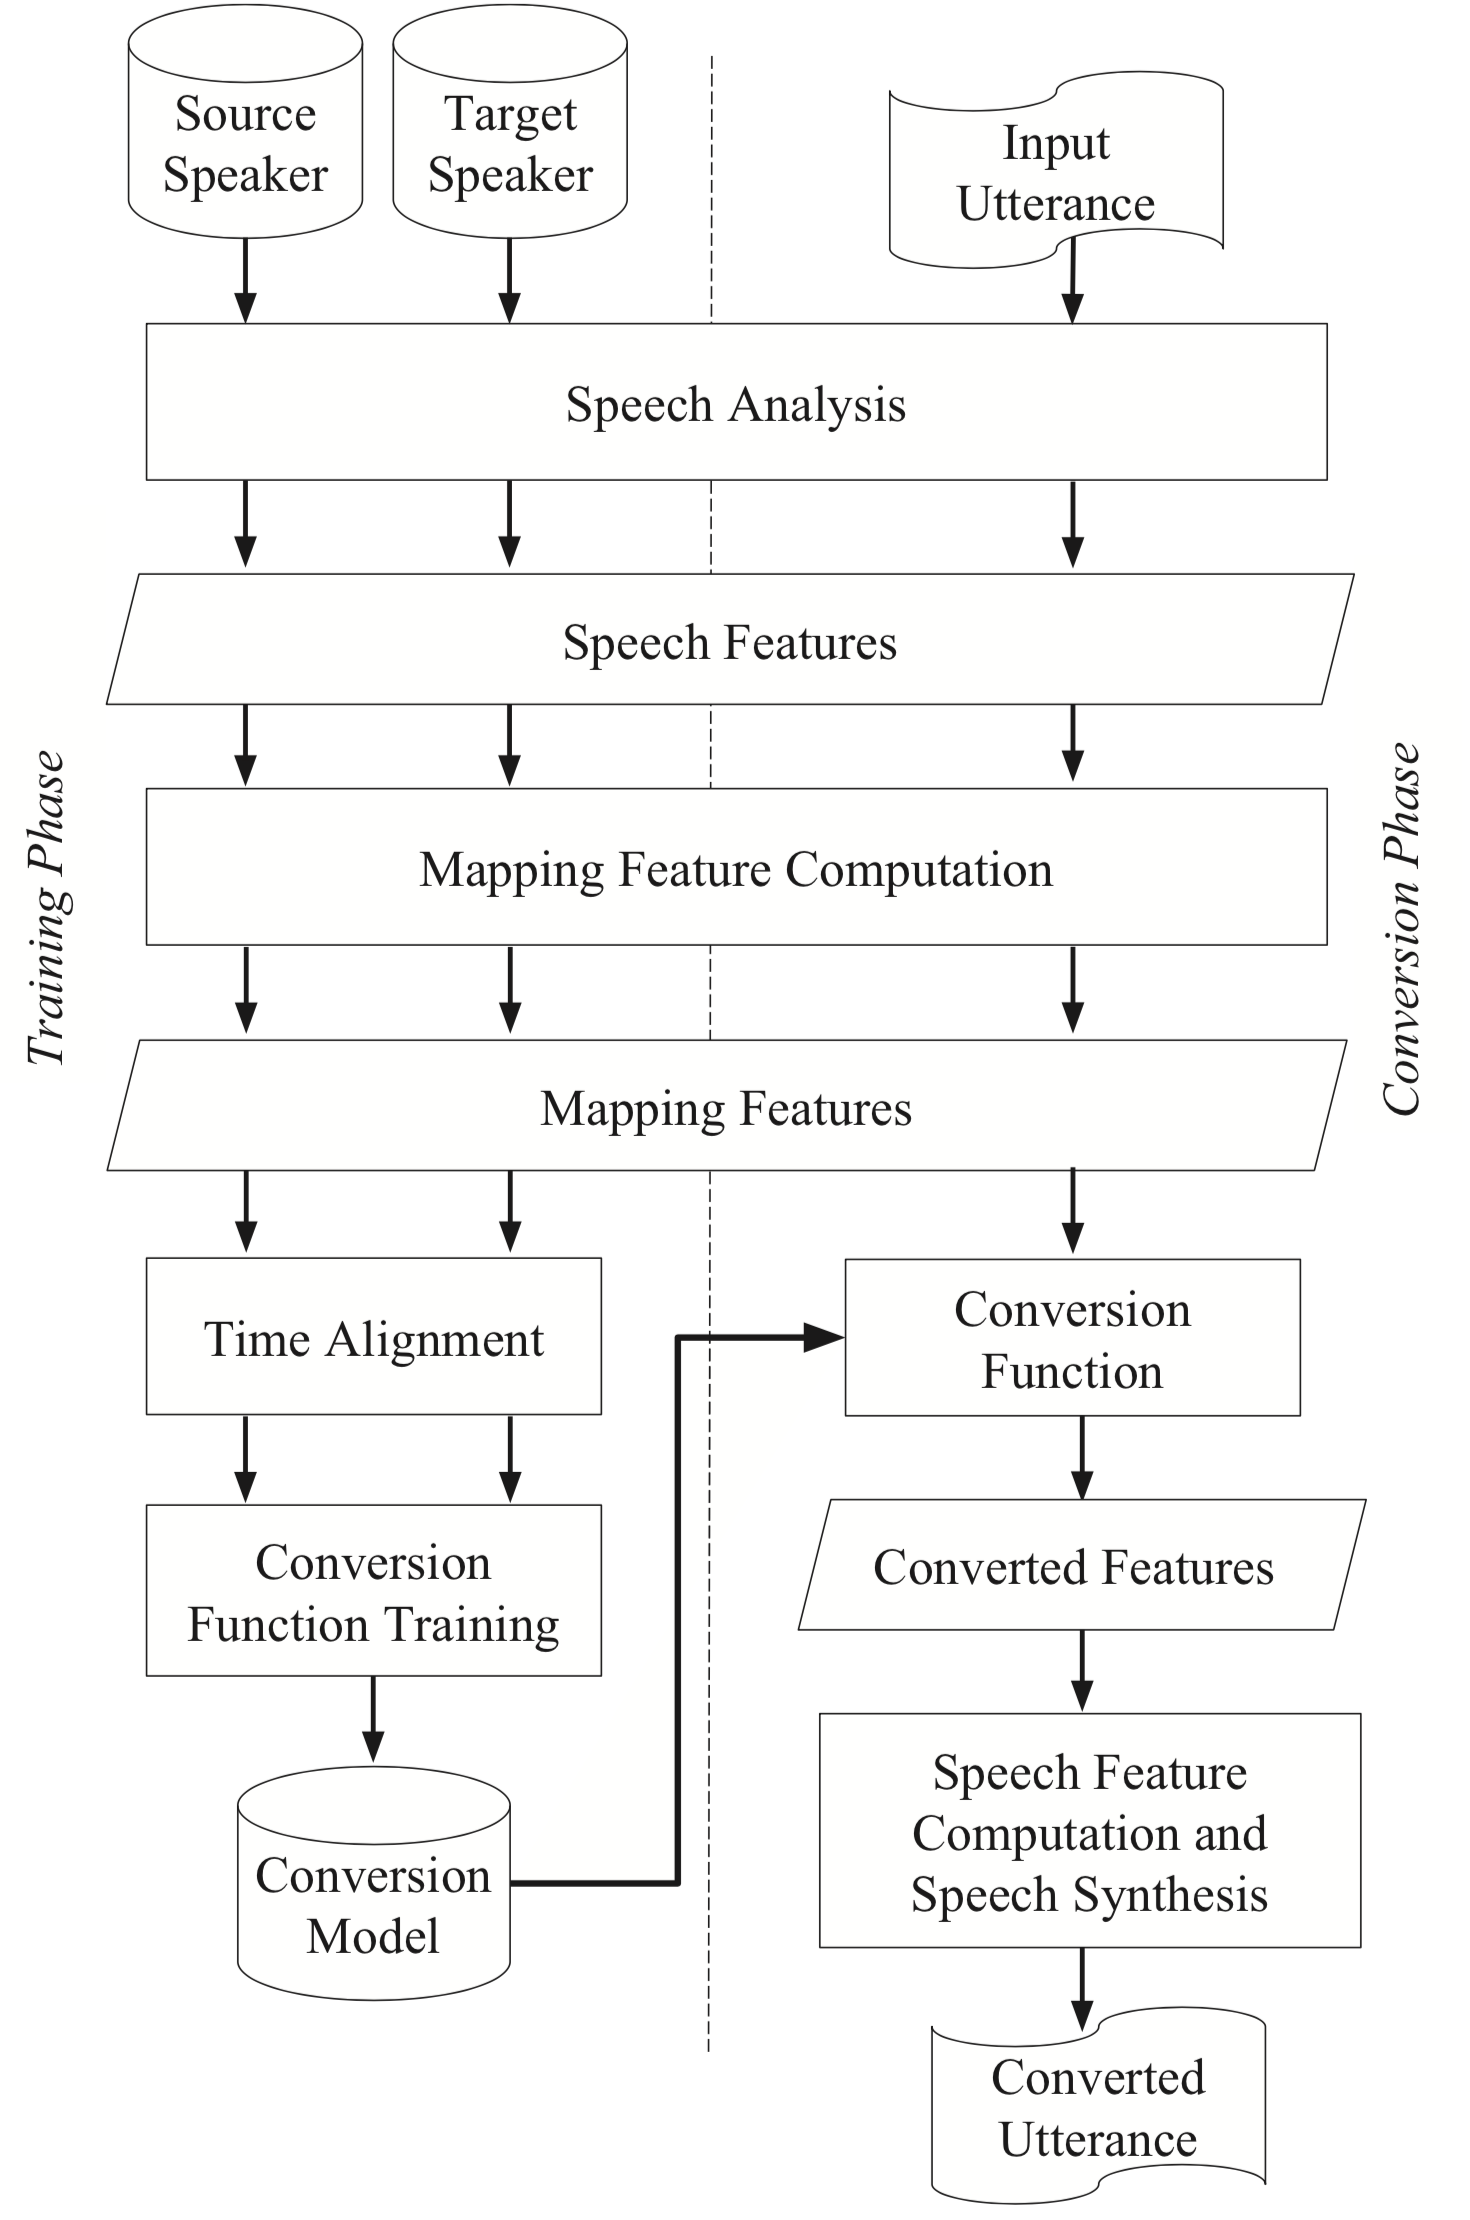
\includegraphics[scale=0.25]{img/vc-flowchart.png}
\caption{The training and conversion processes of a typical VC system.}
\label{fig:vc-flowchart}
\end{figure}

\subsubsection*{Previous works}

There have been a number of efforts to design voice conversion systems
using various methodologies. One particular method that has been applied
recently from other areas of speech technology is the usage of
\emph{i-vectors}. I-vectors are akin to word embeddings in text-based
natural language processing tasks in the sense that i-vectors
encapsulate any type of desired speech information in a vectorized
fashion. In the instance of voice conversion, i-vectors are made of
speaker super-vectors trained on GMMs and low dimensional features that
represent an individual speaker's features \parencite{wu2016}. This is
extracted per utterance and then averaged to form an i-vector that
represents an individual speaker. In this way, a source speaker's
i-vector can be approximated towards a target speaker's i-vector by a
mapping function using neural networks, gaussian mixture models, or
other appropriate algorithms.

The usage of i-vectors in voice conversion has been seen in works such
as \textcite{wu2016} and \textcite{kinnunen2017}. Following
\textcite{kinnunen2017}, the usage of i-vectors in voice conversion
aligns perfectly with the task as it is highly similar to speaker
verification; however instead of being a classification task (e.g.~is
this said speaker or not), voice conversion is a regression task. In
\textcite{wu2016}, they test and compare a variety of frameworks, such
as a deep bi-directional long-short term memory neural (DBLSTM) network
architecture, a DBLSTM combined with an average voice model, a DBLSTM
combined with an average voice model retrained on some paralleled data,
and another model which combined a DBLSTM, average voice model, and
i-vectors. In order to evaluate these models, they provide both an
objective evaluation using a measure known as mel-cepstral distortion
(MCD) and a subjective evaluation rated on quality and similarity, which
was decided by the votes of 20 listeners.

{[}expand on \textcite{wu2016} more{]}

Following the results of the subjective evaluation, they find that
adding i-vectors to the DBLSTM and average voice model outperforms the
DBLSTM and average voice model \emph{without} i-vectors and that the
DBLSTM and average voice model with i-vectors performs almost as well as
the DBLSTM that was retrained. This underscores the need for i-vectors
to capture speaker characteristics; without, the system highly
underperforms and has poor quality and similarity.

As oppose to \textcite{wu2016} which utilizes an \emph{eigenvoice} (or
average voice), \textcite{kinnunen2017} supersedes \textcite{wu2016} by
not requiring \emph{any} parallel data.

Although most voice conversion systems have been successful at the
general task, many of them suffer from low quality and/or low
naturalness in their final outputs. For example, in listening to the
audio of
\textcite{wu2016}\footnote{Visit http://www.nwpu-aslp.org/vc/apsipa-jiewu-demo.pptx to hear samples.}
it is apparent that regardless of the low quality of the original source
and target audios, the quality of the converted audio sounds muffled.
This can be attributed to the various nuanced steps and features
required to have high quality voice conversion.

for example, in a shared task dedicated to voice conversion,
appropriately called \emph{The Voice Conversion Challenge} where many
leading research groups involved in speech technology around the world
have submitted systems in attempts to tackle the issue. In the second
iteration of the challenge \textcite{lorenzo-trueba2018}, the organizers
proposed both a parallel and non-parallel version of the task, both of
which were evaluated on natural and similarity using crowdsourcing.

The type of systems submitted to this year's version of the task
displays the current state of voice conversion and perhaps machine
learning research in general as this year saw a huge increase in the
number of systems using neural networks. However, it does not go without
saying that there were indeed systems that used more traditional
statistical methods, such as Gaussi an Mixture Models (GMM) and one of
its variations, differential GMM (DIFFGMM).

In order to evaluate the systems, a group of roughly 300 listeners were
gathered to carry out a perceptual evaluation. The systems were
evaluated on two main measures: naturalness, which was evaluated on a
scale of 1 (completely unnatural) to 5 (completely natural); and
similarity, which was evaluated using a same/different paradigm.
Following the results, only one system, referred to as N10, was able to
outperform the baseline in terms of naturalness (alongside the original
source and target audios). When observing the performance of other
systems in terms of similarity, we see about 5 our of 23 submitted
systems outperforming the baseline. From this, we can conclude that it
easier to create a system with high similarity than high naturalness,
which is consistent with other common systems.

In discussing the results of the N10 system, the authors credit the
success of the system to the \emph{hundreds of hours} of external speech
data that was utilized to train a model to recognize content-related
features, as well manual fine-tuning. The creators of this system also
made use of WaveNet, a novel high-fidelity vocoder and dozens of hours
of clean English speech, which could also explain the success of their
results. Thus, as previously discussed, we can conclude that creating a
high-fidelity voice conversion requires not only appropriate fine-tuning
of the data, but also a large amount of external data to support the
system.

Thus, even though many systems were neural network based, only one
neural network based system was able to outperform the sprocket
GMM-based baseline, which could suggest that NN-based methods require
proper fine-tuning of the hyperparameters.

Although we see limitations in the systems presented in The 2018 Voice
Conversion Challenge, there have bene other efforts to present high
quality voice conversion systems in works such as and
\textcite{nguyen2016} and \textcite{fang2018}.

\textcite{fang2018} leverages a cycle-consistent adversarial network
(CycleGAN) architecture, a variation of the recently trending generative
adversarial network (GAN) architecture, which was originally used for
unpaired image-to-image translation. For example, GANs have been shown
to be able to convert images of zebras into horses, as well as winter
into summer.

{[}move this paragraph into accent conversion? discuss this as
motivation/inspiration of accent conversion{]} there have also been some
incredible breakthroughs in systems set forth by research teams at
Google Brain. One such system involves the Tacotron end-to-end system,
which has been proposed to replace the current set-up of text-to-speech
systems by reducing the amount of components (decoder, vocoder, etc.
{[}IS THIS TRUE?{]}) into one piece. The researchers working on this
system have recently revealed a impressive system that also takes
advantage of deep neural networks to encode speaker characteristics into
embeddings, which are then utilized to transfer style
\parencite{wang2018}.

With that said, it is evident that the reason for the success of their
systems is due to the availability of large-scale, high quality data
that many research institutions do not have access to or have funding
for. Thus, it may be a long while before the general public has the
ability to replicate such systems; however it is extremely exciting to
know that there is the possibility.

\section{Accent conversion}\label{accent-conversion}

Like voice conversion, accent conversion is dedicated to convert the
speech of a \emph{target speaker} into sounding more like a \emph{source
speaker}. However, accent conversion is specifically focused on morphing
the \emph{accent} of the speech signal, as opposed to sounding directly
like the source speaker. Succinctly stated, ``Accent conversion seeks to
transform second language L2 utterances to appear as if produced with a
native (L1) accent,'' \parencite{aryal2014a}. Accent conversion poses a
further challenge on top of (parallel) voice conversion as the audio of
the source speaker and target speaker is often forced-aligned. This
means that with native and non-native speech, voice conversion would
retain the voice quality and accent of the target speaker
\parencite{aryal2014}.

Due to the specialized nature of accent conversion as compared to voice
conversion, there are fewer articles and systems available for
reference. In fact, most articles that are easily accessible on accent
conversion were all published by the same group of researchers at Texas
A\&M University.

With that said, \textcite{aryal2014} and other works done by the group
of researchers have made efforts to address the challenge. Throughout
their research, they test a variety of methodologies, including accent
conversion through voice morphing and articulatory synthesis. In the
same work of \textcite{aryal2014}, they propose a variation to standard
forced alignment techniques used in voice conversion to pair frames
based on acoustic similarity. To achieve this, they extract 24 MFCCs per
utterance and then dampen the vocal tract differences between the
speakers using a method known as vocal tract length normalization
(VTLN). They then find the closest frames using clusters, which are then
mapped using a GMM conversion method.

In order to evaluate their system, they had a group of 13 participants
rate 12 utterances from the test set for their perceived accent (Which
utterance was less accented?) and perceived speaker identity (Does
utterance X sound more similar to A or B?). This system was compared to
a standard voice conversion system that uses standard forced alignment
and trained using GMMs. They found that comparing the AC system to the
original L2 audio resulted in participants rating the converted audio as
sounding less accented 86\% of the time, while the VC system compared to
the original L2 audio was rated at 91\% of the time. However, when the
converted audios from both systems were compared, participants rated the
AC system to be less accented compared to the VC system 59\% of the
time. It was also concluded that the AC system was more successful in
retaining speaker identity, as the participants found the converted
audio more similar to the L2 speaker 78\% of the time. More
interestingly, they found that the AC system was especially effective in
converted utterances that are harder for the L2 speaker to pronounce.
This was measured by examining the relationship between the number of
phonemes that do not exist in the L2 language (in this case Spanish),
and the number of listeners who judged the converted speech as sounding
less accented.They found that there was a 0.86 correlation, indicating
the robustness of the AC system. Thus, it appears that adjusting the
alignment method to align acoustically similar sounds is a good start
for accent conversion systems.

{[}Add other Aryal papers here{]}

Finally, in \textcite{aryal2015}, we see a more novel method that looks
beyond acoustic features to perform accent conversion.Citing the results
of their previous work, they motivate the usage of articulatory
information in accent conversion reasoning that acoustic-based systems
often struggle in the challenge of separating accent from speaker
identity, which causes the accent converted audio to sound like a
combination of the L1 speaker and L2 speaker. To do this, they propose a
system that combines both the more standard acoustic information like
aperiodicity, pitch and energy from the L1 speaker with articulatory
information recording using an electromagnetic articulograph (EMA). Like
many recent works, they test a DNN-based mapping function between the L1
and L2 data, which they compare to the previously popular GMM-based
system.

In the evaluation of their system, they use crowdsourced efforts to rate
their system based on intelligibility, accentedness, and speaker
identity. They find that the DNN-based system was rated to have a 4.3
out of 7 in terms of intelligibility as compared to 3.84 out of 7 for
the GMM-based system, proving that DNNs are more robust in this
instance. The participants also rated the DNN-based system to be more
native-like in 67\% of cases as compared to the GMM-based system. With
that said, the test set was only 15 sentences, which indicates that 10
out of 15 sentences were better with the DNN system; thus the test set
used may be too small to draw hard conclusions. The most important
conclusions drawn from their experiments was that of the voice identity
assessment. In asking the participants to rate whether an MFCC
compression and AC audio from the DNN and GMM-based systems, they found
that the participants were fairly confident that the two audios were
from the same person with both systems, with the DNN-based system
outperforming the GMM-based system as before at a score of 4.3 out of 7
on average, and the GMM-based system at a score of 4.0. However, this is
difficult to compare to more common acoustic-only accent conversion
systems, as this is not including in their evaluation. With that said,
it may be possible to conclude that this would outperform acoustic-based
systems, as they proposed this system to tackle flaws in their previous
work.

Evidentally, although including articulatory information seems to
improve the performance of accent conversion systems, as discussed in
the closing remarks of their paper, recording articulatory information
can cost a great deal of money and time \parencite{aryal2015}. Most
publically (and privatized) speech corpora also do not include
articulatory information, meaning that experimenting with it in accent
conversion at a broader scale is unfeasibile. Thus, it is ambitious to
accept adding articulatory information to accent conversion systems and
further work needs to be done in order to scale standard audio-based
speech corpora.

Aside from the work done by these researchers, it appears that not much
has been done since to address accent conversion. Looking at their
recent publications, it seems that they have also halted work in this
area, as they have not published articles in the area since 2016; thus
this leaves a gap in the research. However, research in voice conversion
continues to expand, which leaves the potential of apply methodologies
from voice conversion to accent conversion. Following the general
methodologies of voice conversion, I hypothesize that it should be
plausible to convert accents in a similar fashion and apply more recent
innovations to propose state-of-the-art (?!) methods.
\cleardoublepage
\chapter{Design and methodology}

In this chapter, I introduce the dataset and tools utilized in the
experiments, and detail the procedures carried out to conduct the accent
conversion process.

\section{Data}\label{data}

The main dataset utilized in the following experiments is the ABI-1
corpus.

\section{\texorpdfstring{Experiment 1: GMM-based accent conversion-- a
reproduction of
\textcite{aryal2014}}{Experiment 1: GMM-based accent conversion-- a reproduction of }}\label{experiment-1-gmm-based-accent-conversion-a-reproduction-of}

This experiment a) is to understand more traditional mapping methods
used in voice/accent conversion and b) serves as a baseline to be
compared to other innovative methods (e.g Experiment 2).

\section{Experiment 2: I-vector based accent
conversion}\label{experiment-2-i-vector-based-accent-conversion}

This experiment is motivated by the works presented in \textcite{wu2016}
and \textcite{kinnunen2017}. Due to their flexible nature, i-vectors are
an appropriate method to capture the representation of an accent in a
compact way.
\cleardoublepage
\chapter{Experimental results}

In this chapter, I present the results of the experiments described in
the previous chapter and discuss their outcomes and shortcomings.
\cleardoublepage
% \bibliographystyle{apalike-url}
% \renewcommand\bibname{References}
% \nocite{*}
% \bibliography{references}

\printbibliography
\end{document}
